\chapter{Fundamentação Teórica}
\label{cap:fund}

%% - - - - - - - - - - - - - - - - - - - - - - - - - - - - - - - - - - -
\section{Aprendizado por Reforço}
\label{sec:rl}

O Aprendizado por Reforço (RL) é uma abordagem de aprendizado baseada na interação entre um agente e seu ambiente, onde o objetivo principal é maximizar um sinal de recompensa acumulada ao longo do tempo \cite{sutton}. O agente aprende a tomar decisões através de tentativa e erro, ajustando suas ações com base no feedback recebido. Diferentemente do aprendizado supervisionado, que utiliza exemplos rotulados, o aprendizado por reforço explora a recompensa como único sinal de desempenho, lidando com a complexidade de recompensas atrasadas e incertezas na transição de estados. Formalmente, o RL é modelado através de \textbf{processos de decisão de Markov (MDP)}, que definem as interações em termos de estados, ações e recompensas, sendo amplamente aplicável a problemas de decisão sequencial em diversas áreas.

Dentre os métodos avançados de aprendizado por reforço, destaca-se o \textbf{Proximal Policy Optimization (PPO)}, que é amplamente utilizado devido à sua estabilidade em ambientes complexos. Quando aplicado ao \textbf{aprendizado por reforço multiagente (Multi-agent RL)}, permite que diversos agentes aprendam simultaneamente, interagindo de maneira colaborativa ou competitiva. Estratégias como o \textbf{self-play} têm mostrado grande eficácia ao permitir que agentes aprendam uns com os outros em cenários competitivos, como no futebol de robôs. Além disso, o \textbf{curriculum learning} tem sido utilizado para estruturar a aprendizagem progressiva, começando com tarefas simples e avançando para desafios mais complexos, um aspecto crucial em domínios como o \textbf{futebol de robôs}, onde os agentes precisam coordenar habilidades motoras e estratégias de equipe para alcançar um desempenho ótimo.

\subsection{Conceitos Básicos}
\label{subsec:rl_conceitos}

A interação entre o agente e o ambiente é representada esquematicamente na Figura \ref{fig/MDP.png}. O agente observa o estado atual \( S_t \) do ambiente e, com base em sua política de decisão, escolhe uma ação \( A_t \). Após a execução dessa ação, o ambiente evolui para um novo estado \( S_{t+1} \) e retorna ao agente uma recompensa \( R_{t+1} \) associada a essa transição.

\begin{figure}[h]
    \centering
    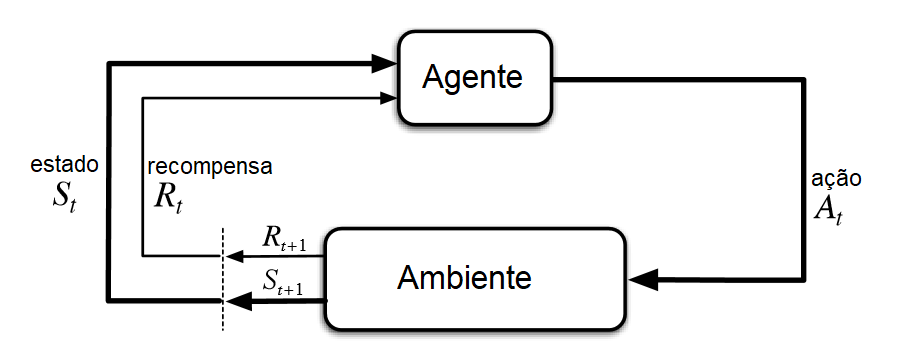
\includegraphics[width=0.6\textwidth]{fig/MDP.png}
    \caption{Interação agente-ambiente no aprendizado por reforço. O agente toma decisões com base no estado atual \( S_t \) e recebe do ambiente uma recompensa \( R_{t+1} \) após realizar a ação \( A_t \).}
    \label{fig:agent_env_interaction}
\end{figure}

\subsubsection*{Elementos Fundamentais:}
\begin{enumerate}
    \item \textbf{Agente e Ambiente:} O agente é a entidade responsável por tomar decisões, enquanto o ambiente é tudo aquilo que responde às ações do agente e fornece feedback.
    \item \textbf{Política (\(\pi\)):} Define a estratégia do agente, especificando a probabilidade de selecionar uma ação específica \( A_t \) em um estado \( S_t \).
    \item \textbf{Sinal de Recompensa (\(R_{t+1}\)):} Indica o valor imediato recebido pelo agente após realizar uma ação. O objetivo é maximizar a soma acumulada das recompensas ao longo do tempo.
    \item \textbf{Função de Valor (\(v(s)\) e \(q(s, a)\)):} Estima o valor esperado da recompensa futura a partir de um estado \( s \) ou de um par estado-ação \( (s, a) \).
\end{enumerate}

\subsubsection*{Exploração vs. Exploração:}
Uma característica central do aprendizado por reforço é o dilema entre explorar novas ações para adquirir conhecimento e explorar o conhecimento atual para maximizar recompensas. O equilíbrio correto entre esses dois aspectos é essencial para o sucesso do agente.

\subsubsection*{Modelagem por Processos de Decisão de Markov (MDPs)}

O aprendizado por reforço é frequentemente modelado por \textbf{Processos de Decisão de Markov} (MDPs, do inglês \textit{Markov Decision Processes}), uma estrutura matemática que captura os aspectos estocásticos e sequenciais da tomada de decisão. Um MDP é definido pelo conjunto quádruplo \((S, A, P, R)\), onde:

\begin{itemize}
    \item \(S\) é o conjunto de estados possíveis do ambiente.
    \item \(A\) é o conjunto de ações possíveis que o agente pode tomar.
    \item \(P(s'|s, a)\) é a probabilidade de transição para o estado \(s'\) dado o estado atual \(s\) e a ação \(a\) tomada.
    \item \(R(s, a)\) é a recompensa esperada ao tomar a ação \(a\) no estado \(s\).
\end{itemize}

O agente busca maximizar a soma esperada das recompensas acumuladas ao longo do tempo, definida pelo \textbf{retorno} \(G_t\). No caso de problemas de horizonte finito, o retorno é dado pela Equação \ref{eq:retorno_finito}:

\begin{equation}
\label{eq:retorno_finito}
G_t = \sum_{k=0}^{T} \gamma^k R_{t+k+1}
\end{equation}

No caso de tarefas contínuas, aplica-se a função de desconto, onde \(\gamma \in [0, 1]\) é o fator de desconto que controla o peso das recompensas futuras, como mostrado na Equação \ref{eq:retorno_infinito}:

\begin{equation}
\label{eq:retorno_infinito}
G_t = R_{t+1} + \gamma R_{t+2} + \gamma^2 R_{t+3} + \dots = \sum_{k=0}^{\infty} \gamma^k R_{t+k+1}
\end{equation}

A modelagem dos MDPs requer duas funções principais de valor, que capturam a expectativa de recompensas futuras:

\paragraph{1. Função de valor de estado (\(v_\pi(s)\)):}
Define o valor esperado de se estar no estado \(s\) e seguir uma política \(\pi\) a partir desse estado, conforme a Equação \ref{eq:valor_estado}:

\begin{equation}
\label{eq:valor_estado}
v_\pi(s) = \mathbb{E}_\pi \left[ \sum_{k=0}^{\infty} \gamma^k R_{t+k+1} \mid S_t = s \right]
\end{equation}

Essa função pode ser definida recursivamente pela \textbf{equação de Bellman}, como mostrado na Equação \ref{eq:bellman_estado}:

\begin{equation}
\label{eq:bellman_estado}
v_\pi(s) = \sum_{a \in A} \pi(a|s) \sum_{s' \in S} P(s'|s, a) \left[ R(s, a) + \gamma v_\pi(s') \right]
\end{equation}

\paragraph{2. Função de valor de ação (\(q_\pi(s, a)\)):}
Define o valor esperado de se tomar a ação \(a\) no estado \(s\) e seguir a política \(\pi\) posteriormente, como apresentado na Equação \ref{eq:valor_acao}:

\begin{equation}
\label{eq:valor_acao}
q_\pi(s, a) = \mathbb{E}_\pi \left[ \sum_{k=0}^{\infty} \gamma^k R_{t+k+1} \mid S_t = s, A_t = a \right]
\end{equation}

Também pode ser escrita de forma recursiva, conforme a Equação \ref{eq:bellman_acao}:

\begin{equation}
\label{eq:bellman_acao}
q_\pi(s, a) = \sum_{s'} P(s'|s, a) \left[ R(s, a) + \gamma \sum_{a'} \pi(a'|s') q_\pi(s', a') \right]
\end{equation}

\paragraph{Equação de Bellman para o Ótimo:}
Para políticas ótimas \(\pi^*\), temos as funções de valor ótimo, dada pela Equação \ref{eq:bellman_otimo_estado}:

\begin{equation}
\label{eq:bellman_otimo_estado}
v^*(s) = \max_a \sum_{s'} P(s'|s, a) \left[ R(s, a) + \gamma v^*(s') \right]
\end{equation}

E a função de valor de ação ótima, apresentada na Equação \ref{eq:bellman_otimo_acao}:

\begin{equation}
\label{eq:bellman_otimo_acao}
q^*(s, a) = \sum_{s'} P(s'|s, a) \left[ R(s, a) + \gamma \max_{a'} q^*(s', a') \right]
\end{equation}

Essas equações de Bellman são fundamentais para algoritmos de planejamento, como \textbf{Value Iteration} e \textbf{Policy Iteration}, mas quando a dinâmica do ambiente não é conhecida, métodos de aprendizado baseados em interação, como Q-learning, se tornam necessários.

Os MDPs constituem o núcleo matemático de muitos algoritmos de aprendizado por reforço, e são essenciais para o desenvolvimento de métodos de otimização de políticas, como o \textbf{Proximal Policy Optimization (PPO)}. Este algoritmo combina exploração e estabilidade ao ajustar políticas dentro de uma região de confiança definida.

\subsection{PPO (Proximal Policy Optimization)}
\label{subsec:ppo}

\subsection{Multi-agent RL}
\label{subsec:marl}

\subsection{Self-play}
\label{subsec:self_play}

%% - - - - - - - - - - - - - - - - - - - - - - - - - - - - - - - - - - -
\section{Curriculum Learning}
\label{sec:curriculum}

\subsection{Conceitos fundamentais}
\label{subsec:curriculum_conceitos}

\subsection{Aplicações em RL}
\label{subsec:curriculum_rl}

\subsection{Estado da arte}
\label{subsec:curriculum_estado_arte}

\subsection{Vantagens e desafios}
\label{subsec:curriculum_vantagens_desafios}

%% - - - - - - - - - - - - - - - - - - - - - - - - - - - - - - - - - - -
\section{Futebol de Robôs}
\label{sec:futebol_robos}

\subsection{Visão geral}
\label{subsec:futebol_visao}

\subsection{Desafios específicos}
\label{subsec:futebol_desafios}

\subsection{Trabalhos relacionados}
\label{subsec:futebol_trabalhos}